% Christian Hubbs
% 28.08.2019

% because I always forget, make sure to run the bibtex command on THIS document!

\documentclass[12pt]{article}
\usepackage[utf8]{inputenc}
\usepackage[english]{babel}
\usepackage{csquotes}
\usepackage{fullpage}
\usepackage{fancyhdr}
\usepackage[pdftex]{graphicx}
\graphicspath{{./images/}}
\usepackage{setspace}
\usepackage{color}
\usepackage{float}
%\hypersetup{draft}
\usepackage{hyperref}
\usepackage{amsmath}
\usepackage{amsfonts}       % blackboard math symbols
\usepackage{nicefrac}       % compact symbols for 1/2, etc.
\usepackage{microtype}      % microtypography
\usepackage{algorithm}
\usepackage{algpseudocode}
\usepackage{lipsum}
\usepackage{booktabs}
\usepackage[margin=1in]{geometry}
\usepackage{subcaption}
\newcommand{\ra}[1]{\renewcommand{\arraystretch}{#1}}
\usepackage{chngcntr} % Adjusts the equation numbering by section
%\counterwithin*{equation}{section}
\newcommand{\norm}[1]{\left\lVert#1\right\rVert} % Provides norms in mathmode
\newcommand{\citetemp}[1]{(#1)}
\usepackage{wrapfig}
\usepackage{hanging}
\newcommand\tab[1][1cm]{\hspace*{#1}}
\usepackage[toc,page]{appendix}
\usepackage{rotating}
\usepackage{multirow}
\newcommand{\textcite}[1]{\citeauthor{#1}, \citeyear{#1}}
\providecommand{\keywords}[1]{\textit{Keywords:} #1}
%\usepackage{biblatex}
\doublespacing
 
%Import the natbib package and sets a bibliography  and citation styles
\usepackage{natbib}
\bibliographystyle{abbrvnat}

\title{OR-Gym: A Reinforcement Learning Library for Operations Research Problems}
\author{
	Christian D.~Hubbs,\thanks{Department of Chemical Engineering, Carnegie Mellon University, Pittsburgh, PA 15123} \\
	Hector D. Perez,\footnotemark[1] \\
	Owais Sarwar,\footnotemark[1]\\
	Nikolaos V. Sahinidis,\footnotemark[1] \\
	Ignacio E. Grossmann,\footnotemark[1] \\
	John M. Wassick\thanks{Dow Chemical, Digital Fulfillment Center, Midland, MI 48667}
}

\begin{document}

\maketitle

\begin{abstract}
We introduce OR-Gym, an open-source benchmark in the form of OpenAI Gym for developing reinforcement learning algorithms to address operations research problems.
Reinforcement learning has been widely applied to game-playing and surpassed the best human-level performance in many domains, yet there are few use-cases in industrial or commercial settings.
We apply reinforcement learning to the knapsack, bin packing, travelling salesman, news vendor, max pooling, portfolio optimization, and vehicle routing problems as well as more general, multi-period resource task networks. 
These problems cover logistics, finance, engineering, and are common in many business operation settings.
In each case, we select a prototypical version from the literature to benchmark reinforcement learning and other optimal approaches against. 
\end{abstract}

\keywords{Machine Learning, Reinforcement Learning, Optimization, Scheduling, Stochastic Programming}

\section{Introduction}

Reinforcement learning (RL) is a branch of machine learning that seeks to make a series of sequential decisions to maximize a reward \citep{Sutton2018}.
The technique has recieved widespread attention in game-playing, whereby RL approaches have beaten some of the world's best human players in Go, DOTA2, and StarCraft II to name a few (\citet{Silver2017}, \citet{Berner2019a}, \citet{Vinyals2019}). 
There is a growing body of literature that is applying RL techniques to existing OR problems.
% Basically took these next few lines from Balaji 2019 for a placeholder 
\citet{Bello2019} applies RL to the travelling salesman problem (TSP) and knapsack problems (KP). 
\citet{Kool2019} apply RL to the TSP and variants such as the vehicle routing problem (VRP) and a prize-collection variant. 
\citet{Nazari2018} solve static and online versions of the VRP.
\citet{Kong2019} use RL to solve an online knapsack problem, secretary and adwords problems.
\citet{Oroojlooyjadid2017} apply RL to the beer game.
\citet{Lin2018} use RL for taxi fleet management. 
% End plagarism
\citet{Balaji2019} provided versions of online bin packing, news vendor, and vehicle routing problems as well as models for RL benchmarks.

Despite these successes only a handful of industrial examples exist in the literature. 
\citet{Hubbs2020} use RL to schedule a single-stage chemical reactor under uncertain demand which outperforms naive optimization models. 
% Add other industrial applications as they may arise. There are some other refs in my paper.

We seek to provide a standardized library for the research community who wishes to extend RL into commercial applications by building on top of the preceding work and releasing OR-Gym, a single library that relies on the familiar OpenAI interface for RL \citep{Brockman2016}, but contains problems relevant for industrial use.
To this end, we have incorporated the benchmarks in \citet{Balaji2019}, while extending the library to address the TSP, KP, portfolio optimization, and multi-period resource task networks (RTN). 
RL problems are formulated as Markov Decision Processes (MDP), meaning they are sequential decision making problems, often times probabilistic in nature, and rely on the current state of the system to capture all relevant information for determining future states. % Can clean up this language a bit.
This framework is not widely used in the optimization community, so we make explicit our thought process as we reformulate many optimization problems to fit into the MDP mold without loss of generality.
Many current RL libraries such as OpanAI Gym, have many interesting problems, but problems that are not directly relevant to industrial use.
Moreover, many of these problems (e.g. the Atari suite) lack the same type of structure as classic optimization problems, and thus are primarily amenable to model-free RL techniques, that is RL algorithms that learn with little to no prior knowledge of the dynamics of the environment they are operating in.
Bringing well-studied optimization problems to the RL community may encourage more integration of model-based and model-free methods to reduce sample complexity and provide better overall performance.
It is our goal that this work encourages further development and integration of RL into optimization and the OR community while also opening the RL community to many of the problems and challenges that the OR community has been wrestling with for decades.

The library itself along with example code to enable reproducibility can be found at \href{www.github.com/hubbs5/or-gym}{www.github.com/hubbs5/or-gym}.

\section{Knapsack}

The Knapsack Problem (KP) was first introduced by \citet{Mathews1896}, and a classic exposition of the problem can be found in \citet{Dantzig1957} where a hiker who is packing his bag for a hike is used as the motivating example.
Obvious applications such as determining what cargo to load into a plane or truck to transport.
Other applications come from finance, we may imagine an investor with limited funds who is seeking to build a portfolio, or apply the framework to warehouse storage for retailers \citep{Ma2019}.

There are a few versions of the problem in the literature, the undbounded KP, bounded, multiple choice, multi-dimensional, quadratic, and online versions \citep{Kellerer2004}.
It is a NP-hard combinatorial optimization problem that seeks to maximize the value of items ($v_i$) with a given non-negative weight ($w_i$) contained in a knapsack subject to a weight limit $W$. 
The problem has been well studied and is typically solved by dynamic programming approaches or via mathematical programming algorithms such as branch-and-bound.

We provide three versions of the knapsack problem, the Unbounded Knapsack Problem (UKP), Bounded Knapsack Problem (BKP), and the Online Knapsack Problem (OKP). 
The first two are deterministic problems where the complete set of items, weights, and values are known from the outset. 
The OKP, is stochastic; each item appears one at a time with a given probability and must be either accepted or rejected by the algorithm.
The online version is studied by \citet{Marchetti-Spaccamela1995}, who propose an approximation algorithm such that the expected difference between this algorithm and the optimal value is, on average, $\mathcal{O}(\textrm{log}^{3/2}n)$. \citet{Lueker1995} later improved this result with an algorithm that closes the gap to within $\mathcal{O}(\textrm{log}n)$ on average, using an on-line greedy algorithm.


\subsection{Unbounded Knapsack}

The unbounded version of the knapsack problem (UPK) can be formulated as an optimization problem as follows:
%
\begin{equation}
\textrm{max} \; z = \sum_{i=1}^n v_i x_i
\end{equation}
%
\begin{equation}
\textrm{s.t.} \; \sum_{i=1}^n w_i x_i \leq W
\end{equation}
%
\begin{equation}
x_i \in \rm \mathbb{Z}^+
\end{equation}
%
\begin{equation}
v_i \in \rm I\!R^+
\end{equation}
%
where $x_i$ denotes a binary decision variable to include or exclude an item from the knapsack. 
This can be solved as an integer programming problem using algorithms such as branch-and-bound to maximize the objective function. 
In the unbounded case, the number of times the algorithm can select a given item is unlimited.

\subsection{Bounded Knapsack}

The bounded knapsack problem (BKP) differs from the unbounded case in that each item can only be selected a limited number of times. 
This introduces an additional constraint into our model shown below in equation \ref{eq:bounding_constraint}.
%
\begin{equation}
\textrm{max} \; z = \sum_{i=1}^n v_i x_i
\end{equation}
%
\begin{equation}
\textrm{s.t.} \; \sum_{i=1}^n w_i x_i \leq W
\end{equation}
%
\begin{equation}
\sum_i x_i \leq N_i
\label{eq:bounding_constraint}
\end{equation}
%
\begin{equation}
x_i \in \mathbb{Z}^+
\end{equation}
%
\begin{equation}
v_i, w_i \in \rm I\!R^+
\end{equation}
%
where $N_i$ is the number of times an item can be selected.

\subsection{Online Knapsack}

A version of the Online Knapsack Problem (OKP) is found in \citet{Kong2019}.
This requires the algorithm to either accept or reject a given item that it is presented with.
There are a limited number of items that the algorithm can choose from and each is drawn randomly with a probability $p_i$. 
After $M$ items have been drawn, the episode terminates leaving the knapsack with the items inside.
The goal here is the same as for the traditional knapsack problems, namely to maximize the value of the items in the knapsack while staying within the weight limit.

\subsection{Benchmark}

The UKP and BKP are solved as integer programs using Gurobi 8.2 and Pyomo 5.6.2 to optimality.
This method will yield the optimal solution for comparison of the RL model. 
Additionally, we will employ a heuristic solution that uses the value to weight ratio of each item to fill the knapsack first with the items that have the highest value to weight ratio before moving to the second item in the list and so forth until the weight limit is reached.
Each of these methods is available within the OR-Gym library.
For UKP we use a simple heuristic given in \textcolor{red}{citation} which selects the next item that fits with the largest value/weight ratio. 
The BKP heuristic modifies the UKP heuristic in one area, it first checks to ensure that the item is available before continuing to maximize the value/weight ratio. 
The OKP algorithm used is a greedy online algorithm based on the TwoBins algorithm given in \citet{Han2015} and is given below in \ref{algo:okp}.
Within the OR-Gym library, the UKP is given by Knapsack-v0, BKP by Knapsack-v1, and the OKP by Knapsack-v2. 

\begin{algorithm}
\begin{algorithmic}[1]
\Require
Choose $r \in [0, 1]$ with equal probability \par
\For{Each item $i \in N$ in order}: \par
    \If{$r=1$}: \par
        \If{$w_i \leq W$}: \par
            Select $i$ for the knapsack \par
        \Else \par
            Reject $i$ \par
        \EndIf \par
    \If{$r=0$}: \par
        \If{$\sum_i^n w_i \leq W$}: \par
            Reject $i$
        \Else \par
            Select $i$ for the knapsack \par
        \EndIf \par
    \EndIf \par
\EndFor \par
\end{algorithmic}
\caption{\footnotesize TwoBins Online Knapsack Algorithm}
\label{algo:okp}
\end{algorithm}

\subsection{Problem Formulation}

While IP solutions seek to solve the problem simultaneously, RL requires a MDP formulation which relies on sequential decision making.
In this case, the RL model must select successive items to place in the knapsack until the limit is reached.
This approach seems more akin to how a human would pack a bag, placing one in at a time until the knapsack is full.
The human knapsack-packer can always remove an item if she determines it does not fit or finds a better item, our RL system, however cannot.
Once an item is selected for inclusion, it must remain (this is made explicit for all algorithms in the OKP case).

The RL system requires a state to make each decision.
In each case, the state could be as simple as the current weight load inside the knapsack, at which point the system would make random selections until it learned a suitable sequence of actions to fill the knapsack.
This approach certainly does not bode well for transfer to new sets of items or knapsacks with different weight limits.
Moreover, the single-state input is wasting potentially valuable information such as the value of the items, the weight, the ultimate carrying capacity of the knapsack, and in the bounded cases, the number of items available to be selected.
For this reason, we provide each of these values as part of the state output.
In the UKP case, the environment returns a tuple of three vectors: item value, item weight, and a vector containing the current load in the knapsack and weight limit.
For the BKP and OKP cases, we add a fourth vector containing the number of items available to be selected.

The reward function for our RL algorithm will simply be the value of each item that is placed within the knapsack for all cases.

\subsection{Reinforcement Learning Algorithm}

Need to select an algorithm here...

\subsection{Results}

\begin{table}
\centering
\caption{Knapsack Results}
\ra{1.3}
\begin{tabular}{@{}lccc@{}}\toprule
%\multirow{2}{opt}{Problem} & Heuristic & IP & RL 
Problem & RL & Heuristic & Optimal \\
\midrule
UKB & 4,800 & 4,800 & 4,800 \\
BKB & 0 & 1,855 & 1,855 \\
OKB\footnote{Results averaged over 100 trials.} & 0 & 253 & 471 \\
\bottomrule
\end{tabular}
\label{tab:kp_results}
\end{table}


\section{Bin Packing}

The Bin Packing Problem (BP) is a classic problem in operations research. 
In its most common form, there are a series of items in a list $i \in I$, each with a given size, $s_i$.
The algorithm must then place these items into one of a potentially infinite number of bins with a size $B$ \citep{Coffman2013}. 
The objective is often to minimize the number of bins used, to minimize the unused space in the bins, or some other, related objective, while ensuring that the bins stay within their size constraints.
We can normalize the bin size to 1 without loss of generality in the case where all bins are of equal size.
For problems with identical bin sizes, we can formulate the problem as:
%
\begin{equation}
    \textrm{min} \; \sum_{j=1}^n y_j
\label{eq:bin_packing_count_obj}
\end{equation}
%
\begin{equation}
    \textrm{s.t.} \sum_{i=1}^m s_i x_{ij}\leq By_j \quad \forall j \in J
\end{equation}
%
\begin{equation}
    \sum_{j=1}^n x_{ij} = 1 \quad \forall i \in I
\end{equation}
%
where $x_{ij}$ are binary assignment variables for each item that must be assigned to a given bin, and where $y_j$ are bins to be opened by the packing algorithm.

Applications of BP's are common in numerous fields, from loading pallets \citep{Ram1992}, to robotics, box packing \citep{Courcoubetis1990}, stock cutting \citep{Gilmore1961}, logistics, and data centers \citep{Song2014}.

BP's are primarily divided into groups based on their dimensionality, although even 1-D problems are NP-hard (\citet{Christensen2017}, \citet{Johnson1974}). 
1-D problems only consider a size or weight metric, whereas multi-dimensional problems consider an item's area, volume, or combination of features. 

\subsection{Problem Formulation}

We provide multiple versions of the bin packing problem in the OR-Gym library, including the environments implemented by \citet{Balaji2019}, which rely on the examples and algorithms provided in \citet{Gupta2012}. 
We refer readers to their work for details and results.
In addition to this environment, we implement multi-dimensional versions of the bin packing problem with data from \citet{Cortez2017}. 
This data was collected over a 30-day period from Microsoft Azure data centers containing multiple physical machines (PM) to host virtual machine (VM) instances.
Each VM has certain compute and memory requirements, and the algorithm must map a VM instance to a particular PM without exceeding either the compute or memory requirement. 
In this case we model the normalized demand at 15-minute increments over a 24-hour period, whereby a new VM instance must be assigned every 15 minutes.
Two versions of this problem are implemented, one involving permanent assignment, and a second, more dynamic problem where the VM instances each have a finite and stochastic duration.

The environment requires mapping of each VM instance to one of 50 PM's at each time step. 
The objective is to minimize unused capacity on each PM with respect to both the compute and memory dimensions for each time step. 
The episode runs for a single, 24-hour period and ends if the model exceeds the limitations of a given PM.
At each time step, the agent can select from one of the 50 PM's available.
If a selection causes a PM to become overloaded, the agent incurs a large penalty and the episode ends.
It is important to ensure that the penalty is sufficiently large to prevent the agent from ending the episode prematurely, otherwise the agent will find a locally optimal strategy by simply ending the episode as quickly as possible.
Given that RL does not use constraints in the traditional sense, these types of penalties need to be used in order to provide ``soft constraints'' so that the agent can learn an acceptable policy.
It is also possible to mask PM's from the action space that would be overloaded if they were to be selected.
This may more closely represent a hard constraint, but it is not clear how that would affect learning.

\subsection{Benchmark}

Heuristics such as Best Fit (BF) \citep{Johnson1974}, and Sum of Squares (SS) \citep{Csirik2006}, have been proposed and are well studied, providing theoretical optimality bounds in the limit for one-dimensional BP's. 
For multi-dimensional problems, other heuristics such as Next Fit Decreasing Height (NFDH) and First Fit Decreasing Height (FFDH) are early and common heuristics approximation ratios of 3 and 2.7 respectively \citep{Christensen2017}. 
Currently, \citet{Bansal2016} provides the best results in the 2-D case with an asymptotic approximation guarantee of $\approx 1.405$.
We use employ the FirstFit algorithm for the 2-D bin packing case with no rotation as described in \cite{Garey1972} to compare our RL approach with.
The FirstFit algorithm is given below and was shown to have an asymptotic performance ratio of 1.7 \citep{Baker1983}.

\begin{algorithm}
\begin{algorithmic}[1]
\Require
Initialize environment with $J$ empty bins.\par
\For{Each item $i \in I$ in order}: \par
    \For{Each open bin $j \in J$ in order}: \par
        \If{$i$ fits in bin $j$}: \par
            Place item $i$ in bin $j$ \par
        \EndIf \par
    \EndFor \par
    \If{$i$ does not fit into any open bin}: \par
        Open new bin. Place item into new bin. \par
    \EndIf \par
\EndFor
\end{algorithmic}
\caption{\footnotesize FirstFit VM Packing Algorithm}
\label{algo:ff_vmpacking}
\end{algorithm}

The optimization model solves the VM packing problem deterministically, off-line to provide an upper bound on performance. As in the standard case, the objective is to minimize the total number of bins (or physical machines) in use for all time steps. The full model is given below.

\begin{equation}
    \textrm{min}\; \sum_{i=1}^M  \sum_{k=1}^T \bigg( \sum_{j=1}^N x_{ijk} (D_j^{mem} + D_j^{cpu} \big) \bigg) - 2 z_{ik}
\label{eq:vm_packing_obj}
\end{equation}

\begin{equation}
    \textrm{s.t.} \sum_j D_j^{mem} x_{ijk} \leq B_{mem} \quad \forall j \in N, k \in T
\end{equation}

\begin{equation}
    \sum_j D_j^{cpu} x_{ijk}  \leq B_{cpu} \quad \forall j \in N, k \in T
\end{equation}

\begin{equation}
    \sum_k^T x_{ijk} \leq \tau_j y_{ij} \quad \forall i \in M, j \in N
\end{equation}

\begin{equation}
    \sum_{j=1}^N y_{ij} = 1 \quad \forall i \in M
\end{equation}

\begin{equation}
    \sum_j^N x_{ijk} \leq 1 \quad \forall k \geq t \in T 
\end{equation}

\begin{equation}
    z_{ik} \geq x_{ijk} \quad \forall i \in M, j \in N, k \in T
\end{equation}

where $i$, $j$, and $k$ are indices that denote the physical machine in the set $M$, the virtual machine requirements in $N$, and the time step in $T$ respectively. $D_j^{mem}$ and $D_j^{cpu}$ indicate the memory and CPU demand for each VM instance, which lasts for time $\tau$. Each physical machine may host multiple processes simultaneously, but these are restricted by normalized memory and compute capacities, denoted by $B_{mem}$ and $B_{cpu}$ respectively. 

The model also makes use of multiple binary, decision variables, $x$, $y$, and $z$. $x$ maps VM's to PM's for each time period. $y$ relates VM's to PM's, while $z$ enables the time periods of the PM's to be linked and used in the objective.

\subsection{Results}

\section{Newsvendor}

The Newsvendor Problem (NVP) is a classic problem that describes a vendor's daily decision on how many newspapers to purchase each day for resale. The difficulty in the decision is that the vendor faces an uncertain demand each day. Any unsold papers are lost since it is assumed that any excess inventory at the end of the day is worthless for the next day (who wants to buy yesterday's newspaper?). However, if the vendor knew what probability distribution the demand was coming from, the critical fractile formula could be used to determine the optimal order quantity, $q$. The inputs to this formula are the inverse cumulative distribution function of the demand $F^{-1}$, the newspaper unit purchase cost $c$ and the newspaper unit sales price $p$.

\begin{equation}
    q = F^{-1}\left(\frac{p-c}{p}\right)
\end{equation}

This classical problem can be extended to describe the multi-period inventory problem in a multi-echelon supply chain (Fig. \ref{fig:supplychain}). The following description is for a single product system. However, the problem can be extended to a multi-product system if desired. In the single product system, it is assumed that the product is non-perishable and sold in discrete quantities. Stage 0 has the retail site, which is an inventory location that sells the product to external customers. Each other stage has both an inventory area and a manufacturing area. The inventory is used as feed to the manufacturing area to produce an intermediate of the final product. The ratio of inventory to intermediate produced is 1:1. Material produced at a stage is transferred to the inventory area of the stage below it. Transfer of material can be subject to lead times. Each manufacturing site has a limited production capacity. Each inventory holding area also has a limited holding capacity. The last stage has access to an unlimited supply of raw materials and no inventory is held at this stage.

\begin{figure}[h]
    \centering
    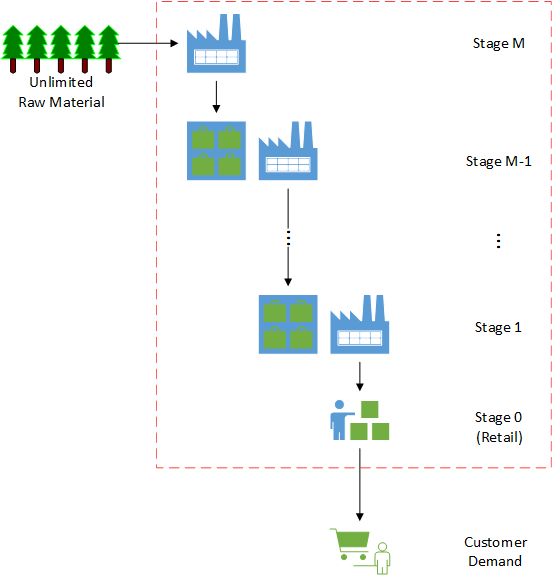
\includegraphics[width=0.7\textwidth]{SupplyChain.png}
    \caption{Multi-echelon inventory-production supply chain}
    \label{fig:supplychain}
\end{figure}

At each time period in the NVP, the following sequence of events occurs:
\begin{enumerate}
    \item Stages 0 through M-1 place replenishment orders to their respective suppliers. Replenishment orders are filled
        according to available production capacity and available inventory at the respective suppliers. It is assumed that production is relatively fast and material is sent to the next stage before step 2.
    \item Stages 0 through M-1 receive incoming inventory replenishment shipments that have made it down the product pipeline
        after the respective lead times.
    \item Customer demand occurs at stage 0 (retailer).
    \item Demand is filled according to available inventory at stage 0.
    \item One of the following occurs,
        \begin{enumerate}
            \item Unfulfilled sales and replenishment orders are backlogged at a penalty. 
            Note: Backlogged sales take priority in the following period.
            \item Unfulfilled sales and replenishment orders are lost with a goodwill loss penalty.
        \end{enumerate}
    \item Surpluss inventory is held at each stage at a holding cost.
\end{enumerate}

Any inventory remaining at the end of the last period is lost.

There are six governing equations for the NVP. The first two (Equations \ref{eq:invbal} - \ref{eq:pipebal}) are material balances for the on hand ($I$) and pipeline ($T$) inventory at the beginning of each period $n$, respectively. The on hand inventory at each stage $m$ in the beginning of the next period is equal to the initial inventory in the current period, plus the reorder quantity arrived ($R$, placed $n-L_m$ periods ago), minus the sales in the current period ($S$). The pipeline inventory at each stage in the beginning of the next period is equal to the pipeline inventory in the current period, minus the delivered reorder quantity (placed $n-L_m$ periods ago), plus the current reorder quantity placed. Equation \ref{eq:reorder} relates the accepted reorder quantity ($R$) to the requested reorder quantity ($\hat{R}$). In the absence of capacity ($c$) and inventory constraints in the stage above the current stage, the accepted reorder quantity would be equal to the requested order quantity plus the backlog from the previous time point. However, when these constraints exist, the place an upper bound on the reorder quantity that is accepted. At stage $|\mathcal{M}|-1$, the term $I^{m+1}_n$ can be ignored or set to $\infty$. 

Equation \ref{eq:sales} gives the sales $S$ at each period, which equal the reorder quantity from the stage below on stages $1$ through $|\mathcal{M}|$ and equal to the fulfilled customer demand at the retailer (stage $0$). The fulfilled customer demand is equal to the demand plus the previous period backlog, unless there is insufficient on hand inventory at the retailer. The unfulfilled demand $U$ or unfulfilled reorder requests is given by Equation \ref{eq:unfulfilled}. It should be noted that $\hat{R}^{-1}_n \equiv D_n$. The profit $P$ is given by Equation \ref{eq:profit}, which discounts the profit (sales revenue, minus procurement costs, minus unfulfilled demand costs, minus excess inventory holding costs) with a discount factor $\alpha$. $p$, $r$, $k$, and $h$ are the unit sales price, unit procurement cost, unit penalty for unfulfilled demand, and unit inventory holding cost at each stage $m$, respectively. For stage $|\mathcal{M}|$, $R^m_n \equiv S^m_n$ and $r^m$ represents a production cost, instead of a procurement cost. If backlogging is not allowed, any unfulfilled demand or procurement orders are lost sales and all $B$ terms are set to 0.

\begin{align}
    & I^m_{n+1} = I^m_n + R^m_{n-L_m} - S^m_n && \forall m \in \mathcal{M}, n \in \mathcal{N} \label{eq:invbal} \\
    & T^m_{n+1} = T^m_n - R^m_{n-L_m} + R^m_n && \forall m \in \mathcal{M}, n \in \mathcal{N} \label{eq:pipebal} \\
    & R^m_n = \min\left(c^{m+1},I^{m+1}_n,\hat{R}^m_n + B^{m+1}_{n-1}\right) && \forall m \in \mathcal{M} \setminus \{|\mathcal{M}|\}, n \in \mathcal{N} \label{eq:reorder} \\
    & S^m_n = 
    \begin{cases}
        R^{m-1}_n & \text{if $m>0$}\\
        \min\left(I^0_n + R^0_{n-L_m},D_n + B^0_{n-1}\right) & \text{if $m=0$}
    \end{cases}
    && \forall m \in \mathcal{M}, n \in \mathcal{N} \label{eq:sales} \\
    & U^m_n = \hat{R}^{m-1}_n + B^m_{n-1} - S^m_n && \forall m \in \mathcal{M}, n \in \mathcal{N} \label{eq:unfulfilled} \\
    & P^m_n = (\alpha)^n \cdot \left(p^m S^m_n -  r^m R^m_n - k^m U^m_n - h^m I^m_{n+1}\right) && \forall m \in \mathcal{M}, n \in \mathcal{N} \label{eq:profit}
\end{align}

\subsection{Problem Formulation}

\subsection{Benchmark}

The base stock policy has been shown to be optimal for capacitated production-inventory systems under certain conditions (\cite{Kapuscinski1999OptimalSystems}). For multi-stage systems, these conditions are that backlogging is allowed (no lost sales), lead times are fixed, and the capacity at a stage does not exceed the capacity at the stage below it. Although the base-stock policy is not necessarily optimal under other conditions, it is chosen as the benchmark for the NVP due to its simplicity. Under this policy, the requested reorder quantity is given by Equation \ref{eq:basestock}, where $z^m$ is the base-stock level at stage $m$ and the term in the summation is the inventory position in period $n$.  

\begin{equation}
    \hat{R}^m_n = \max\left(0,z^m - \sum_{m^\prime = 1}^m \left(I^{m^\prime}_n + T^{m^\prime}_n - B^{m^\prime}_{n-1}\right)\right)
    \label{eq:basestock}
\end{equation}

\cite{Glasserman1995SensitivitySystems} propose a numerical method to determine the optimal base-stock level called infinitesimal perturbation analysis (IPA). IPA is a gradient descent approach that minimizes the expected cost over a sample path. In the present work, we follow this idea of optimizing over a sample path (either offline or online), but use more robust approaches for the optimization. Since objective function for the NVP (normalized expected profit over the sample plath, Equation \ref{eq:samplepath}) is non-smooth and non-differentiable for discrete demand distributions, line search algorithms based on the Wolfe conditions (\cite{Nocedal2006NumericalOptimization}) often fail to converge when determining the step size for the IPA approach. Thus a derivative-free optimization (DFO) approach and a mixed-integer programming (MIP) approach are used instead. 

\begin{equation}
    f = \frac{1}{|\mathcal{N}|} \mathbf{E}_D \left[\sum_{m\in \mathcal{M}} P^m_n\right]
    \label{eq:samplepath}
\end{equation}

The first approach is to use Powell's Method (\cite{Powell1964AnDerivatives}), which does not rely on gradients and can be applied to non-differentiable systems. Powell's method is implemented using the minimize routine within the Scipy Optimize module in Python (\cite{Virtanen2020SciPyPython}). The negative of the objective function in Equation \ref{eq:samplepath} is used since we are minimizing instead of maximizing. Since the demand distributions are discrete, Powell's Method is followed by a local search to find the nearest optimal integer solution. Enumeration is used to compare all neighboring integer solutions to the optimum found by Powell's method. The second approach is to model the NVP system using mixed-integer linear programming and optimize the base-stock levels using a MIP solver. The disjunctions arising from the minimum operators in Equations \ref{eq:reorder} - \ref{eq:sales}, and \ref{eq:basestock} are reformulated into algebraic inequalities using Big-M reformulations (Equations \ref{eq:max} - \ref{eq:max3}). Furthermore, to ensure the standard multi-echelon condition $z^m \leq z^{m+1} \; \forall m \in \mathcal{M} \setminus |\mathcal{M}|$, the base stock levels are written in terms of the total inventory level, $x^m \geq 0$, at each stage ($z^m = \sum_{m^\prime = 1}^m x^{m^\prime}$).

\begin{align}
    x = \max(A_1,...,A_n) \qquad \qquad \label{eq:max}\\
    A_i \leq x \leq A_i + M_i(1-y_i) \qquad \forall i \label{eq:max1} \\
    x = \min(A_1,...,A_n) \qquad \qquad \label{eq:min} \\
    A_i + M_i(1-y_i) \leq x \leq A_i \qquad \forall i \label{eq:min1} \\
    \sum_{i=1}^n y_i = 1 \qquad \qquad \qquad \label{eq:max2} \\
    y \in \{0,1\}^n \qquad \qquad \qquad \label{eq:max3}
\end{align}

\subsection{Reinforcement Learning Algorithm}

\subsection{Results}

Two examples are run to compare the OR and RL approaches in the NVP. Example 1 is a 90 period 4 stage supply chain with backlog. A Poisson distribution is used for the demand with the distribution mean at 20. A discount factor for the time value of money of 97\% percent is used (3\% discount). The stage specific parameters used in Example 1 are given in Table \ref{tab:nvp_example1}.

Example 2 is identical to Example 1, but no backlogging is allowed (all unfulfilled request are considered lost sales).

\begin{table}[!h]
    \centering
    \caption{Parameters values in Examples 1 and 2}
    \label{tab:nvp_example1}
    \begin{tabular}{ccccc}
    \toprule
    Parameter & Stage 0 & Stage 1 & Stage 2 & Stage 3 \\ \midrule
    $I_0$     & 100     & 100     & 200     & -       \\
    $p$       & \$2.00  & \$1.50  & \$1.00  & \$0.75  \\
    $r$       & \$1.50  & \$1.00  & \$0.75  & \$0.50  \\
    $k$       & \$0.10  & \$0.075 & \$0.05  & \$0.025 \\
    $h$       & \$0.15  & \$0.10  & \$0.05  & -       \\
    $c$       & -       & 100     & 90      & 80      \\
    $L$       & 3       & 5       & 10      & -       \\ \bottomrule
    \end{tabular}
\end{table}

\begin{figure}[!h]
    \centering
    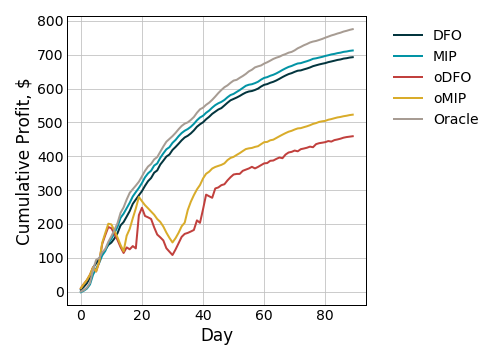
\includegraphics[width=0.7\textwidth]{NewsVendor_Backlog.png}
    \caption{Cumulative profit in NewsVendor Example 1}
    \label{fig:NV_backlog}
\end{figure}

\begin{figure}[!htbp]
    \centering
    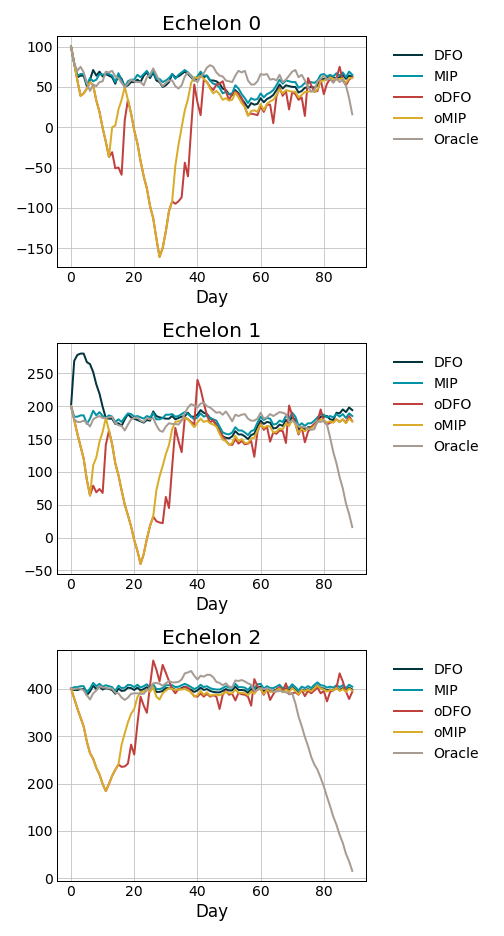
\includegraphics[width=0.7\textwidth]{NewsVendor_Backlog_inventory.png}
    \caption{Total inventory levels in NewsVendor Example 1}
    \label{fig:NV_backlog_inv}
\end{figure}

\begin{figure}[!htbp]
    \centering
    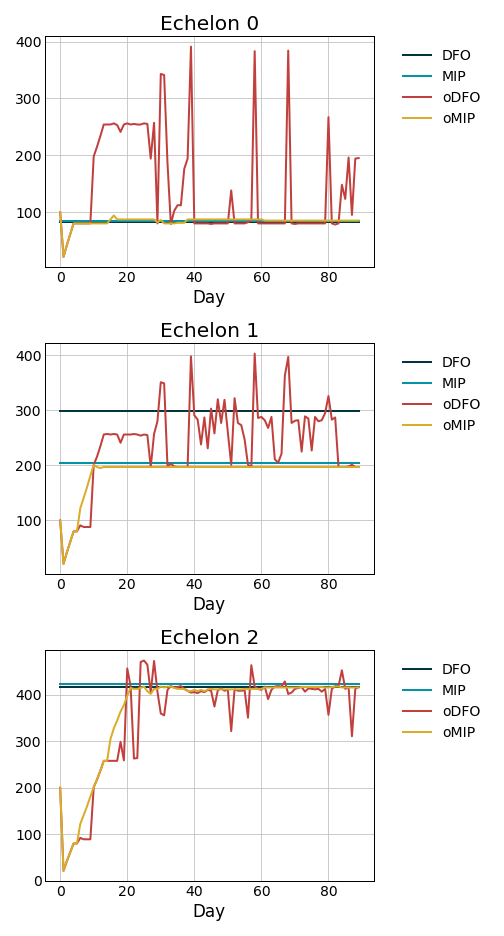
\includegraphics[width=0.7\textwidth]{NewsVendor_Backlog_zopt.png}
    \caption{Optimal base stock-levels in NewsVendor Example 1}
    \label{fig:NV_backlog_basestock}
\end{figure}

\begin{figure}[!h]
    \centering
    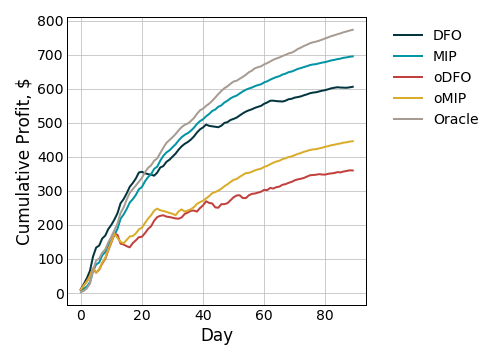
\includegraphics[width=0.7\textwidth]{NewsVendor_LostSales.png}
    \caption{Cumulative profit in NewsVendor Example 2}
    \label{fig:NV_LostSales}
\end{figure}

\begin{figure}[!htbp]
    \centering
    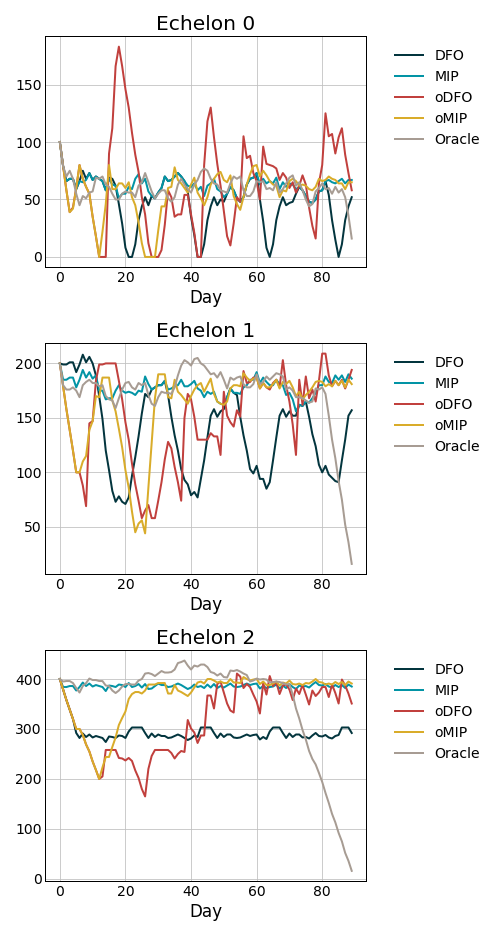
\includegraphics[width=0.7\textwidth]{NewsVendor_LostSales_inventory.png}
    \caption{Total inventory levels in NewsVendor Example 2}
    \label{fig:NV_LostSales_inv}
\end{figure}

\begin{figure}[!htbp]
    \centering
    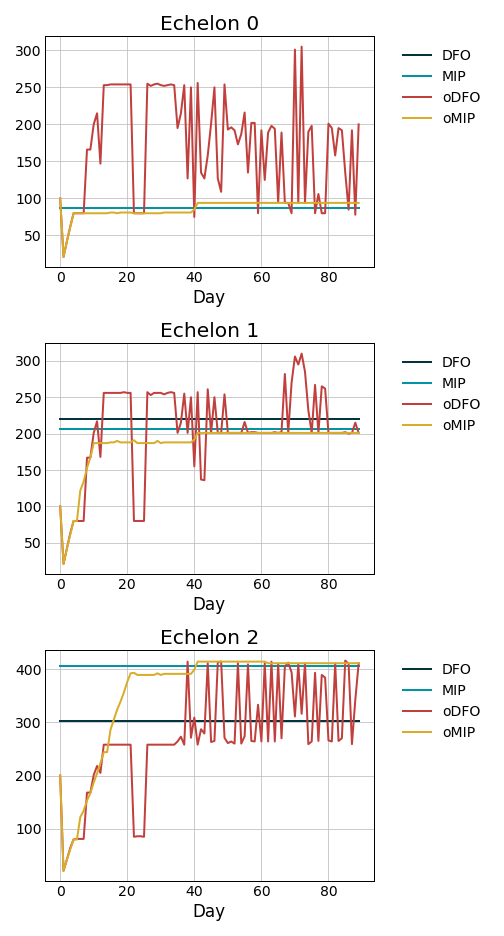
\includegraphics[width=0.7\textwidth]{NewsVendor_LostSales_zopt.png}
    \caption{Optimal base stock-levels in NewsVendor Example 2}
    \label{fig:NV_LostSales_basestock}
\end{figure}

\section{Vehicle Routing}

A classic challenge in combinatorial optimization, first proposed in 1959 by Dantzing and Ramser, the vehicle routing problem (VRP) is the task of determining the optimal route of a fleet of vehicles from their origin depot(s) to sets of customers across space and time \cite{Dantzig1959}. 
There are different variations of the VRP including the Capacitated VRP where there is a limit on the capacity of the vehicle and the VRP with Time Windows where customers must be visitied during a particular time interval, among many others \citep{PIllac2013}. 
These VRP can additionally be either static or dynamic and either deterministic or stochastic. 



\subsection{Problem Formulation}

\lipsum[1]

\subsection{Benchmark}

\subsection{Reinforcement Learning Algorithm}

\subsection{Results}

\section{Portfolio Optimization}

Portfolio optimization (PO) refers to the task of creating a collection (portfolio) of financial assets as to maximize an investors return, subject to some investment criteria and constraints. The most famous approach to PO stems from Markowitz's mean-variance framework from the 1950s that models portfolio optimization as a trade-off between the return of an asset (modeled using its expected value) and the risk associated with the asset (modeled by its variance) \cite{Markowitz1952}. 
Since then, the PO problem has been extensively explored in the literature with a multitude models that take into account many different practical considerations. 

\subsection{Problem Formulation}
Here, we focus on the \textit{multi-period asset allocation problem} of \citet{Dantzig1993}. 

An investor starts with a portfolio $\mathbf{x}^0 = [x^0_1,...,x^0_n]$ consisting of $n$ assets, with an additional quantity of cash we call a `zero' asset, $x_0^l$. The investor wants to determine the optimal distribution of assets over the next $L$ periods to maximize her total wealth at the end of the final investment period $L$.

The optimization variables are $b_i^l$ (the amount of asset $i$ bought at the beginning of period $l$) and $s_i^l$ (the amount sold) where $i=1,...,n$ and $l=1,...,L$. 

The price of an asset $i$ in period $l$ is denoted by $P_i^l$. We assume that the cash account is interest-free meaning that $P_0^l = 1, \forall l$. The sales and purchases of an asset $i$ in period $l$ are given by proportional transaction costs $\alpha_i^l$ and $\beta_i^l$, respectively. These prices and costs are subject to change asset-to-asset and period-to-period. 

The deterministic version of this problem is given by Formulation \ref{eq:DetPOFormulation}: 

\begin{subequations}\label{eq:DetPOFormulation}
\begin{align}
    \max_{\mathbf{x},\mathbf{s},\mathbf{b}} \sum_{i=0}^n P_i^L x_i^L \label{eq:POobj} \\
    x_0^l \leq x_0^{l-1} + \sum_{i=1}^n (1-\alpha_i^l) P_i^l s_i^l - \sum_{i=1}^n (1+\beta_i^l) P_i^l b_i^l \quad \forall l = 1,...,L \label{eq:PObal} \\
    x_i^l = x_i^{l-1} - s_i^l + b_i^l \quad \forall i = 1,...,n \quad \forall l = 1,...,L \label{eq:POsum}\\
    s_i^l, b_i^l, x_i^l \geq 0 \quad \forall i = 0,...,n \quad \forall l = 1, ..., L\label{eq:POnonneg}
\end{align}
\end{subequations}
\subsection{Benchmark}
\cite{Ben-Tal2000}. 
\subsection{Reinforcement Learning Algorithm}

\subsection{Results}

\section{Conclusion}

\subsection{Future Work}

\newpage

\bibliography{references.bib}

\end{document}

